% to run: lualatex ttZ_EFT.tex
\RequirePackage{luatex85}
\documentclass[tikz, border=10pt]{standalone}

\usepackage[compat=1.1.0]{tikz-feynman}

\newcommand{\Ptop}{\ensuremath{\mathrm{t}}}
\newcommand{\Pg}{\ensuremath{\mathrm{g}}}
\newcommand{\Pb}{\ensuremath{\mathrm{b}}}
\newcommand{\Pq}{\ensuremath{\mathrm{q}}}
\newcommand{\PH}{\ensuremath{\mathrm{H}}}
\newcommand{\PW}{\ensuremath{\mathrm{W}}}
\newcommand{\PZ}{\ensuremath{\mathrm{Z}}}

\makeatletter
\tikzset{
  position/.style args={#1 degrees from #2}{
    at=(#2.#1), anchor=#1+180, shift=(#1:\tikz@node@distance/1.1)
  }
}
\makeatother

\begin{document}
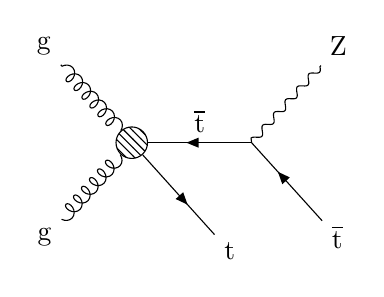
\begin{tikzpicture}
  \begin{feynman}
    \diagram [arrow size=1pt, horizontal=a to b] {
      i1 [particle=\(\Pg\)] -- [gluon] a [blob, minimum size=0.4cm] -- [gluon] i2 [particle=\(\Pg\)],
      a -- [anti fermion, edge label=\(\overline \Ptop\)] b,
      o1 [particle=\(\PZ\)] -- [boson] b -- [anti fermion] o2 [particle=\(\overline \Ptop\)],
    };

    \vertex [position=-48 degrees from a] (c) {\(\Ptop\)};

    \diagram* [arrow size=1pt] {
      (c) -- [anti fermion] (a);
    };
  \end{feynman}
\end{tikzpicture}
\end{document}
